
\section{Grundlagen}

Hier erklären was kommt

\subsection{Microservices}

Für den Begriff Microservices existiert keine einheitlich anerkannte Definition. Während Wolff unter Microservices unabhängig, deploybare Module versteht\cite{wolff2018mic_praxis}, spricht Newman von kleinen, autonomen Services, die zusammenarbeiten. Cockcroft verwendet den Begriff Microservice gekoppelt mit einem Architekturbegriff: Eine Microservice Architektur sind gekoppelte Services, welche für einen gewissen Kontextbereich zuständig sind.\cite{irakli2016mic_arc} D.h. jeder Service behandelte gewisse, fachliche Aufgaben und kann genau für diese genutzt werden. Eine Vielzahl von solchen Services bildet dann die gesamte Anwendung. \\

Amudsen schreibt dem Microservice an sich die Eigenschaft zu, dass er unabhängig zu anderen Microservices sein muss, d.h. ein Microservice kann losgelöst von anderen geupdated (deployed) werden. Weiter ist ein Microservice wie schon bei Cockcroft für einen gewissen Aufgabenbereich zuständig. Eine Microservice-Architektur ist ein zusammenschluss von miteinander kommunizierenden Microservices.\cite{irakli2016mic_arc} \\

In \textit{Flexible Software Architecture}\cite{wolff2016mic_architectures} werden Microservices zu den bisherigen noch weitere, teils technische Eigenschaften zugeschrieben: Microservices sind technologisch unabhängig, d.h. eine Microservice Architektur ist beispielsweise nicht an eine bestimmte Programmiersprache oder Datenbank gebunden. Weiter müssen Microservices einen privaten Datenspeicher haben und sie kommunizieren mit anderen Services über das Netzwerk (z.B. über REST). Ebenfalls werden Microservices verwendet, um große Programme in kleine Teile zu unterteilen. Diese kleine Teile lassen sich automatisch bauen und deployen. \\

Basierend auf den folgenden Definitionen wird der Microservice Begriff wie folgt verwendet: Microservices sind
\begin{itemize}
	\item klein in der Größe
	\item kommunizieren mit anderen Services über Netzwerkschnittstellen (z.B. REST) sind unabhängig voneinander deploybar
	\item können unabhängig voneinander entwickelt werden (d.h. Microservice A muss nicht auf B,C,D … warten und/oder umgekehrt)    
	\item eingeschränkt in ihrer Geschäftslogik, d.h. ein Microservice kümmert sich immer um einen speziellen Kontext, der im vorhinein definiert werden muss
	\item dezentral, d.h. sie können auf unterschiedlichsten Plattformen gehosted werden werden automatisch gebaut und deployed
\end{itemize}

Abschließend handelt es sich um eine Microservice-Architektur, wenn viele Microservices nach Definition verwendet werden. 

\subsection{Monolithische Struktur }

Eine monolithische Struktur ist ein einziges Softwareprogramm (Monolith), welches in sich geschlossen ist. Dies bedeutet im Detail, dass ein Monolith aus mehreren Ebenen besteht auf die über Schnittstellen zugegriffen werden kann. Innerhalb der Ebenen werden Komponenten wie z.B. Frameworks oder selbstgeschriebene Klassen eingebunden und verwendet.\cite{msfussell2017azure} Durch die sich aufeinander aufbauenden Ebenen folgt daraus, dass sämtliche Geschäftslogiken, User Interfaces sowie die Datenbank und Datenbankzugriffe Abhängigkeiten haben. All dies ist in einem Programm vereint.\cite{msfussell2017azure} Natürlich kann die monolithische Struktur innerhalb noch einmal Modular sein. In einem Monolithen existierten also ggf. mehrere Module, welche verschiedene Geschäftslogiken abbilden oder ein Modul, welches nur zum Erstellen einer grafischen Oberfläche verwendet wird. Dennoch können diese Module nicht unabhängig von der gesamten Anwendung deployed werden.\cite{nhiem2017mic_moving}

\begin{figure}[ht]
	\centering
	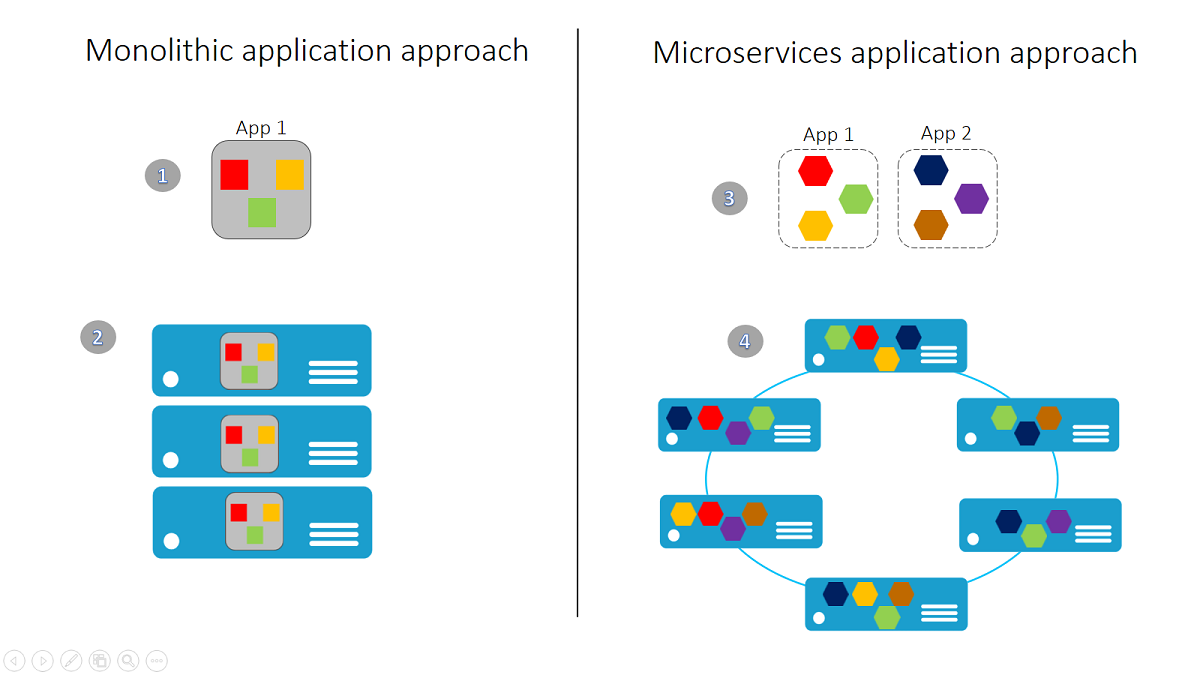
\includegraphics[width=0.9\textwidth]{monolithic_vs_micro}
	\caption{Monolith und Microservice-Architektur.\cite{msfussell2017azure}}
	\label{fig:mono}
\end{figure}

Abbildung \ref{fig:mono} zeigt eine vereinfachte Gegenüberstellung der beiden Architekturen. Die App 1 ist in drei klassische Funktionen (Web, Business und Data) unterteilt. Die Skalierung (2) kann durchgeführt werden, in dem App 1 über mehrere Server oder VMs geklont wird. 

Bei der Microservice Architektur werden die Funktionen auf unterschiedliche Dienste aufgeteilt. Konkreter könnte dies bedeuten, dass App 1 bei (3) zuständig für eine Benutzerkontoverwaltung ist und App 2 für ein Abrechnungssystem. Die Microservices (4) werden nicht geklont, sondern können unabhängig voneinander bereitgestellt werden. 

%TODO: ggf. kommt das in die Konzept-Sektion
\subsection{Monolith vs. Microservices}
Aus den vorherigen Abschnitten sind diverse Unterschiede zwischen den Architekturen erkennbar. Nun gilt es festzustellen, für welche Problemstellungen, welche Architektur sinnvoller ist. \cite{wolff2016mic_architectures} \cite{birk2016mic_soa}  

% Tabelle ist nicht ganz Inhaltich richtig

\begin{center}
	\begin{tabular}{p{5cm}p{5cm}p{5cm}}
		& Monolithische Architektur & Microservice-Architektur \\ \hline
		Abhängigkeiten & alles in einer Anwendung & entkoppelt, da Prinzip von Modularisierung verwendet wird \\
		Größe & linear steigend & einzelne Services sind klein \\
		Geschwindigkeit Zugriffe & schnell, da alles in einer Anwendung & Zugriffe können länger dauern \\ 
		Deployment & schwieriger desto größer das Projekt, aufgrund von
		\begin{itemize}
			\item Abhängigkeiten  
			\item Größe \end{itemize}
		 & einfach, da Microservices \begin{itemize}
			\item klein und 
		    \item modular sind \end{itemize} \\
		Organisation & leichter, da alles an einem Ort & schwerer, da mehr Domänenlogik (wer macht was?) beachtet werden muss \\
		Legacy-Systeme ablösen & ggf. schwierig, da System sehr verzahnt miteinander & leicht, da Microservices durch neue abgelöst werden können \\
		Technologie & beschränkt & vielfältig \\
		Nachhaltige Entwicklung & wartbar mit Einschränkungen & leicht wartbar \\
		Robustheit & weniger, da ganzes System bei schweren Fehlern abstürzt & sehr, da im Zweifel immer nur ein Service abstürzt \\
		Skalierung & horizontale und vertikale Skalierung, Umsetzung kann sehr komplex werden &  horizontale und vertikale Skalierung \\
		Betrieb & nur ein System & komplex, da mehr Services verwaltet werden müssen
	\end{tabular}
\end{center}


Aus der Tabelle ergeben sich verschiedene Punkte: Der Monolith eignet sich besonders dann sehr gut, wenn die Projekt- sowie Teamgrößen absehbar sind und auch die Technologie entschieden ist. Zusätzlich kann es beim Projektanfang ein Vorteil sein, da die Abhängigkeiten innerhalb des Projektes liegen und so Entwicklungsgeschwindigkeit nicht durch komplizierte Infrastrukturen blockiert wird. 
Ist die Projektgröße allerdings nicht absehbar, treten früher oder später mehrere Schwierigkeiten auf: Zum einen bindet der am Anfang des Projektes festgelegte Technologiestack und die Nutzung oder der Austausch neuer Technologien sind in der Regel mit sehr viel Arbeit verbunden. Des Weiteren führen die anfangs eingegangen Abhängigkeiten zu problemenen im Deployment (A kann erst updaten, wenn B soweit ist) und einem erhöhten Aufwand in der Kommunikation zwischen den Teams (A kann erst beginnen, wenn B xy erledigt hat). \\

Zusätzlich ist die Skalierung von Microservices unabhängiger. Es können sich feingranular Services gesucht werden, welche skaliert werden sollen. Diese benötigen nicht zwingend mehr Hardware (vertikale Skalierung), sondern könnten z.B. auch auf verschiedene Server verteilt werden (horizontale Skalierung). Dies ist bei einem Monolithen natürlich auch möglich, dennoch muss immer der ganze Monolith skaliert werden, welcher zum einen immer mehr Hardware als einzelne Microservices benötigt und zum anderen auch durch die Komplexität in der Regel auch schwerer zu skalieren ist.\cite{wolff2018mic_praxis}   
Als abschließender Punkt ist die Robustheit zu erwähnen: Wenn ein Microservice einen Fehler enthält, stürzt dieser im schlechtesten Fall ab. Im besten Fall übernimmt dieser Service eine weniger wichtige Funktion und der Nutzer bemerkt den Ausfall noch nicht einmal. Beim Monolithen dagegen stürzt die gesamte Anwendungen ab. In der Regel startet so eine Anwendung automatisch neu, jedoch ist betrifft die Downtime alle Nutzer. \\

Aus den genannten Punkten lässt sich schließen, dass eine generelle Aussage, ob eine monolithische oder Microservice-Architektur besser oder schlechter ist, sich nicht treffen lässt. Es kommt immer drauf an, welche Zielsetzung und wie viele Ressourcen für das Projekt festgelegt sind. REWE Digital beispielsweise hat ihr Produkt zuerst als Monolithen gestartet und ist erst später auf eine Microservice-Architektur umgeschwenkt.\cite{rewe2019mic_ppp} Zwei mögliche Gründe könnten dafür sein, dass zum einen ein lauffähiges Produkt schneller mit einer monolithischer Struktur zu erreichen ist, zum anderen ist nicht gegeben, ob ein entwickeltes Projekt überhaupt die Nachfrage erzeugt, so dass eine Microservice-Architektur notwendig ist. Dementsprechend muss abgewogen werden, welche Architektur für welchen Anwendungsfall besser geeignet ist.\cite{wolff2018mic_praxis} 

\subsection{Macro und Mikroarchitektur}

Wie bereits erwähnt, ist die Entkopplung von Microservices ein großer Vorteil gegenüber dem Monolithen. Dennoch ist es sinnvoll Richtlinien, Regeln und/oder Festlegungen zu schaffen, damit die Microservices nicht blockierend oder technologisch unnötig gegensätzlich arbeiten. Die Entscheidungsebene kann global (Makroarchitektur) oder nur für einen einzelnen Services (Mikroarchitektur) gelten.\cite{wolff2016mic_architectures} Welche Festlegungen und mit welcher Strenge diese eingehalten werden müssen, hängt von verschiedenen Faktoren ab, welche technologisch, organisatorisch oder wirtschaftlich motiviert sein können.\\ 

In dem folgenden Abschnitt werden Grundprinzipien der Software-Modellierungs-Methodik Domain Driven Design erläutert und im Zusammenhang mit den Begriffen Bounded Context, Makro- und Mikroarchitektur gesetzt sowie gängige Bereiche daraufhin untersucht, ob sie makro- oder microarchitektonisch einzuordnen sind.\\

Domain Driven Design (DDD) ist ein Vorgehen mit dem ein Softwaresystem modelliert werden kann. Im Sinne einer Microservice-Architektur kann dies als Werkzeug genutzt werden, um Microservices fachlich einzuteilen.\cite{heise2016ddd} Beim sogenannten \textit{Strategic Design} wird dafür das Softwaressytem in verschiedene \textit{Bounded Contexts} eingeilt, welche an ein \textit{Domänenmodell} gebunden sind. Ein Domänenmodell bildet die Geschäftslogik ab, d.h. inwiefern einzelne Objekte innerhalb des Kontexts in Relation zueinander stehen, welche Eigenschaften sie haben und wie sich verhalten. Dabei kann ein Domänenmodell - je nach Entwurfsmuster - von einem oder mehreren Bounded Contexts genutzt werden wie in Abbildung XXX zu sehen ist.\cite{wolff2018mic_praxis}  \\

%TODO: drei Bilder einfügen S. 20
%Könnte zu abstrakt sein. Ggf. den Begriff Domänenmodell weiter ausbauen oder einfach ein Beispiel nennen

Wolff verdeutlicht das Prinzip von Bounded Contexts mit Hilfe von vier Microservices, welche einen Onlineshop repräsentieren: \textit{Suche}, \textit{Check Out}, \textit{Inkasso} und \textit{Lieferung}. Während das Datenmodell der Suche detaillierte Informationen über die Produkte enthält, reicht es im Warenkorb (hier Check Out), wenn ggf. nur der Produktname gespeichert wird. Bei Inkasso ist es ähnlich: An dieser Stelle sind Zahlungsdaten des Benutzers relevant, während bei Lieferung die ggf, nur Adresse notwendig ist.\cite{wolff2018mic_praxis} An diesem Beispiel wird deutlich, dass zwar von selben Begrifflichkeiten wie Benutzer, Produkt usw. gesprochen wird, allerdings jeder Service sein eigenes Domänenmodell hat. Durch diese Technik, was dabei hilft, eine saubere Microservice-Architecktur zu erstellen.\cite{wolff2018mic_praxis} \cite{heise2016ddd} \\

Neben der fachlichen Trennung bildet DDD auch die Kommunikation zwischen Kontexten ab. Dabei wird grundsätzlich vom \textit{up-stream} (vorgeschaltet) und dem \textit{down-stream} (nachgeschaltet) gesprochen.\cite{wolff2018mic_praxis} \\

%Hier noch kurz erläutern%
%Auf die unterschieldichen Pattern gehe ich jetzt nicht mehr ein% 
%%% TODO: Upstream und Downstream erklären, andere Entwurfsmuster anreißen, aber nicht besonders ausführen

%das ist Ziel/Abschließender Satz zu DDD %
Nach dem Anwenden von DDD sollte man eine Übersicht haben, welche Microservices benötigt werden und welche Abhängigkeiten sie zu anderne haben.  

%%  Taktisches Design wird nicht erwähnt, whrs. auch viele andere Sachen nicht, das muss ich in der Einleitung für DDD noch erwähnen. 

%% Ggf. noch als Beispiel, aber hier vllt ein wenig unpassend.
I%n Abbildung \ref{fig:rewe_microservice_ui} skizziert REWE Digital, wie viele unterschiedliche Microservices bei dem Anzeigen einer Produktdetailseite bereits involviert sind. \\ 

%\begin{figure}[ht]
%	\centering
%	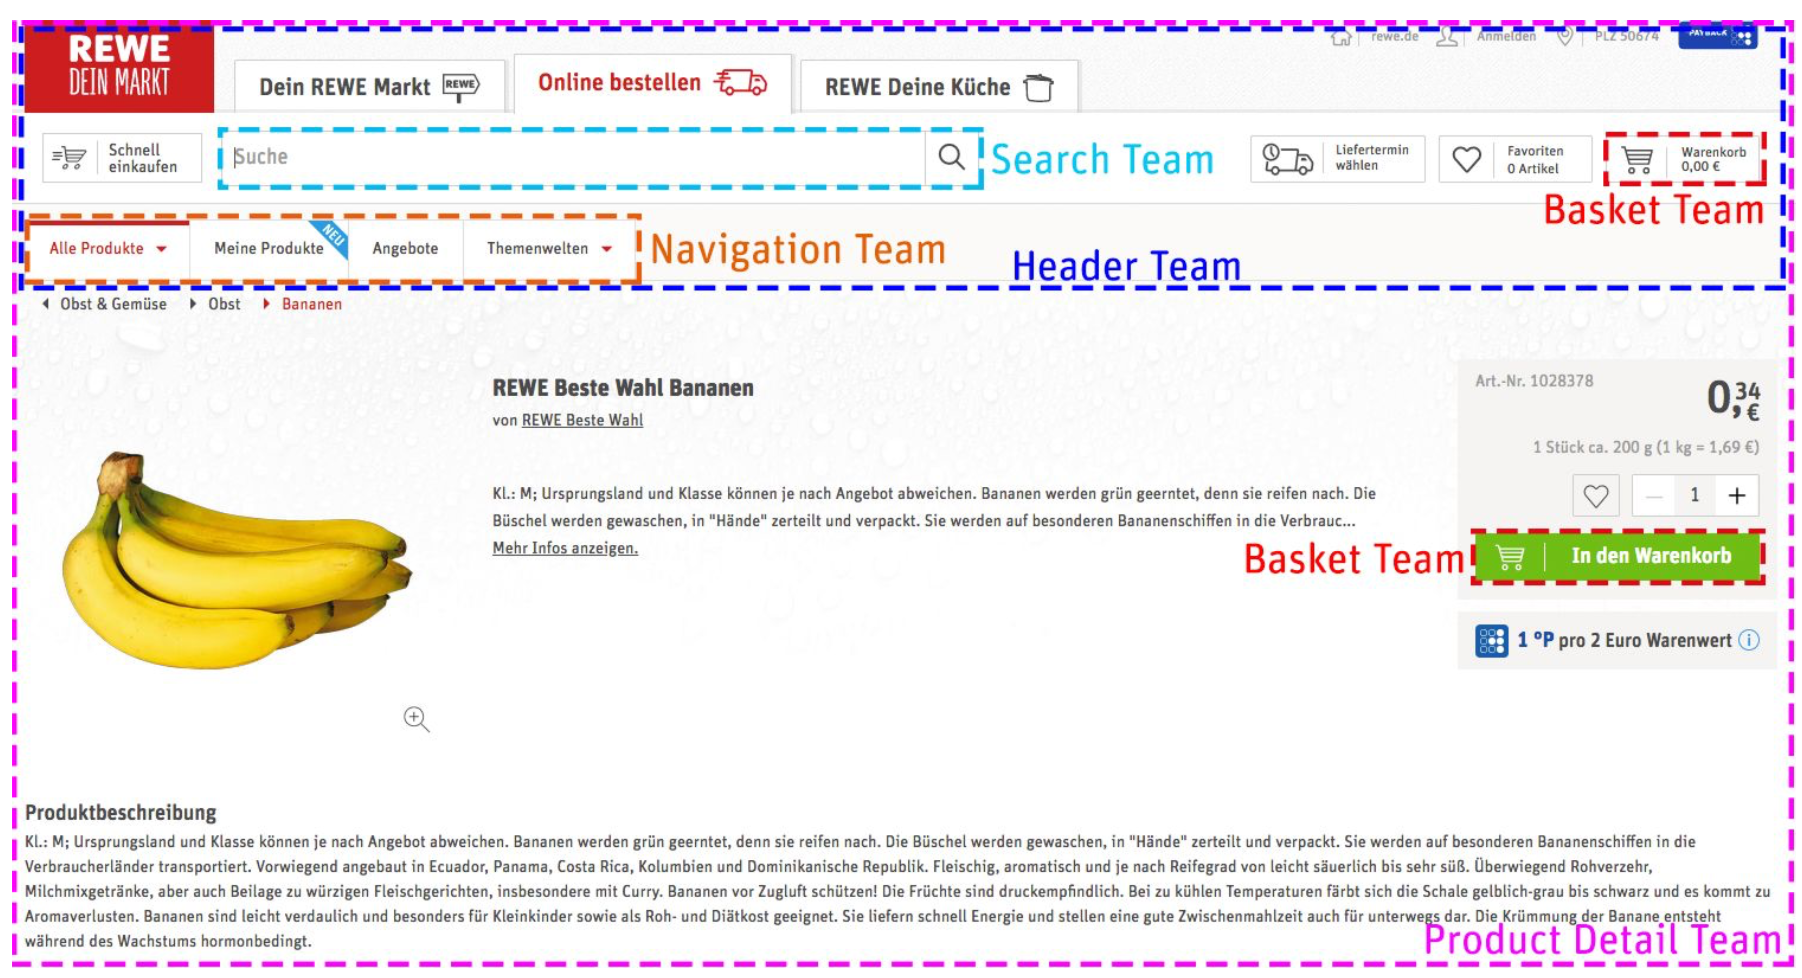
\includegraphics[width=0.9\textwidth]{rewe_digital_front_page}
%	\caption{Aufteilung, welche Microservices, welchen Part in der UI übernehmen.\cite{rewe2019mic_ppp}}
%	\label{fig:rewe_microservice_ui}
%\end{figure}

%Natürlich lässt sich aus der Abbildung \ref{fig:rewe_microservice_ui} nicht schließen, wie das/die Domänenmodell/e aufgebaut ist/sind, aber die zahlreichen Services lassen darauf schließen, dass jeder Service andere Informationen benötigt und das Domänenmodell anders aufbereitet sein wird. 

%Anhand der Abbildung \ref{fig:rewe_microservice_ui} ist gut zu erkennen, dass jeder Service verschiedene Verantwortungsbereiche hat, z.B. die Produktsuche (hellblau), die Warenkorbverwaltung (rot) oder Navigation (orange). Es wäre zwar auch denkbar, einen Bounded Context zu entwerfen, der direkt mehrere Aufgaben (z.B. Suche und Produktdetails) zusammenfasst, allerdings birgt das die Gefahren von einer monolithischen Struktur und würde sich entsprechend negativ auswirken.\cite{wolff2018mic_praxis} \\




%% Auf API Gateway eingehen
